\chapter{Implementation and Results}
In this section we cover the implementation of the project and the results.
As outlined in the Objectives section we can divide the tasks into three main
parts: transmission, optical conversion ,and reception. 
In this project we looked at using a FPGA board for the generation and
reception of the PRBS data.  Hence the overall design is of a board in a
loopback configuration as shown in Figure~\ref{fig:loopback}.

\begin{figure}[ht]
    \centering
    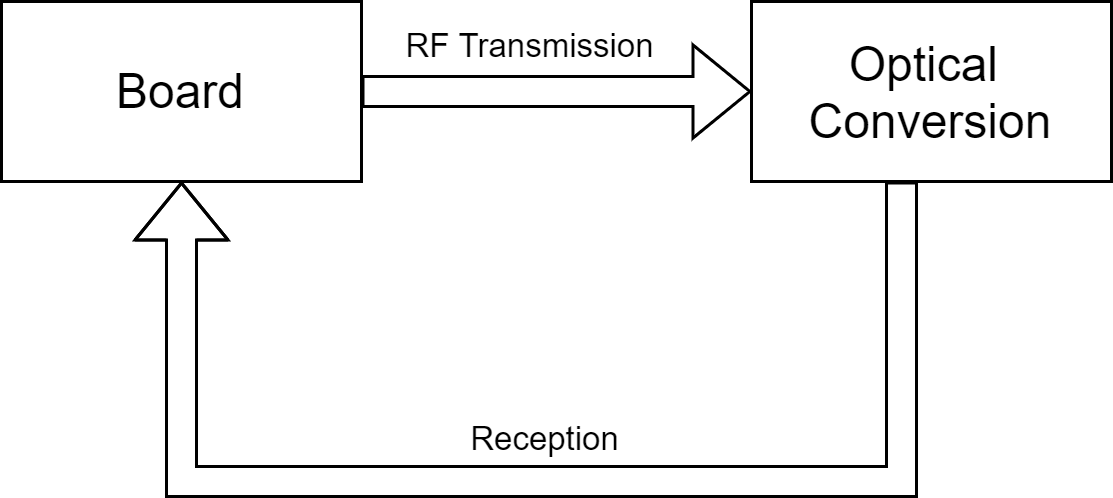
\includegraphics[width=0.5\linewidth]{img/loopback.png}
    \caption{Loopback Configuration}%
    \label{fig:loopback}
\end{figure}

\section{Transmission and Reception}%
\label{sec:transmission_and_reception}




\subsection{Hardware}%
\label{sub:hardware}
To generate and receive PRBS data the VCU118 board was used. The transmission
and reception of the data was handled by the onboard high-speed parallel to
serial GTY transceivers in conjuction with a Si5345 external clock. To connect
with the transceiver the HiTechGLobal FMC-MSMP module was used.
\begin{figure}[ht]
    \centering
    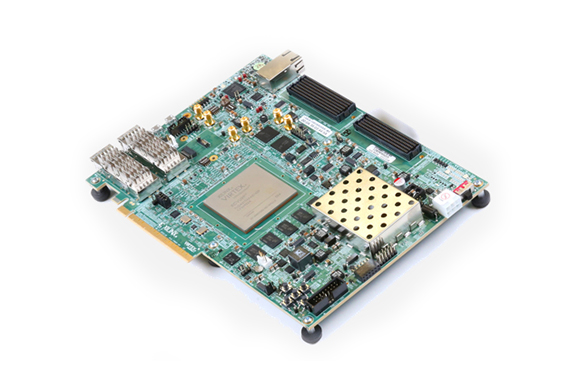
\includegraphics[width=0.5\linewidth]{img/board.jpg}
    \caption{VCU118 Board}%
    \label{fig:board}
\end{figure}

\begin{figure}[ht]
    \centering

    \begin{minipage}[b]{0.6\textwidth}
        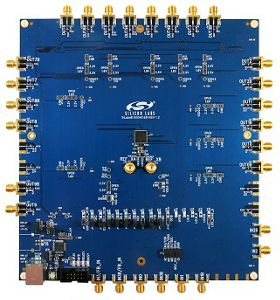
\includegraphics[width=0.8\linewidth]{img/clock.jpg}
        \caption{Si5345 Clock}%
        \label{fig:clock}
    \end{minipage}
    \hfill
    \begin{minipage}[b]{0.3\textwidth}
        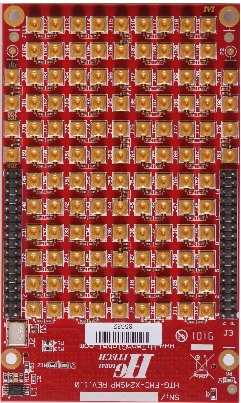
\includegraphics[width=0.8\linewidth]{img/fmc.png}
        \caption{FMC-MSMP module}%
        \label{fig:fmc}
    \end{minipage}

\end{figure}

\subsection{Transceiver Setup}%
\label{sub:transceiver_setup}
Most of the project took place using the transceivers in a simple RF loopback
configuration (no optical transmission).

The setup of the transceivers followed the example design outlined in the user
guide to the transceivers \cite{wizard_guide}. Places where choices were made
(as the example design is not specific to a particular board) or the
design was deviated from are outlined below. 

\subsubsection{Selection of Quads}%
\label{ssub:selection_of_quads}
The GTY transceivers in the VCU118 are grouped into four channels or quads.
Seven GTY quads on the left side of the device and six GTY quads on the right
side of the device.
There are 52 transceivers on VCU118 board, in total.
\begin{itemize}
    \item Four of the GTY transceivers are wired to Samtec Firefly Module Connector 
    \item Four of the GTY transceivers are wired to QSFP1 module connector 
    \item Four of the GTY transceivers are wired to QSFP2 module connector 
    \item Sixteen of the GTY transceivers are wired to the PCIe 16-lane edge connector
    \item Twenty-four of the GTY transceivers are wired to FMC+ HSPC connector
\end{itemize}

As the we were using a FMC-HSMP module, we were limited to the transceivers wired
to the FMC+ HSPC connector.
Furthermore only certain quads can be driven through an external clock - also
there are limitations to the number of quads that can be driven with an
external clock while still meeting jitter requirments, but as we are only
driving two transmitters, it was not an issue.
As such we chose Quad 120 and Quad 122 as the quads for testing.

\subsubsection{Pin Configuration}%
\label{ssub:pin_configuration}
For a full pinout diagram, it is necessary to refer to the user guide of the
board \cite{vcu118_guide}. However the pin choices made are outlined in the
following table.


\subsubsection{Transceiver Configuration}%
\label{ssub:transceiver_configuration}
The transceivers were programmed to run at a standard rate of 10GB/s, with a
reference clock of 156.25 MHz. The free-running clock (used to drive resets)
was driven at 125 MHz, sourced from the onboard 300 MHz system clock. 
The reset functions were bound to the physical push buttons BE23 and BB24. 
Status indicators (Link Up and Link Down) were bound to LED1 and LED0
respectively. 

At the current stage there was no encoding in the setup as we were trying to
troubleshoot an issue with the PRBS checking module. However if running the
system for a long period of time, encoding would be necessary to ensure the CDR
remained locked.
The full details of the setup can be found in
Appendix~\ref{cha:transceiver_settings}.


\subsection{Transmitter}%
\label{sub:transmitter}
In Figure~\ref{fig:transmitter_block} we see a block diagram of the transmitter
(TX) of the transceiver. Parallel data flows into the transmitter interface,
and is seriallised, then finally flows out of the transmitter as high-speed
serial data.

\begin{figure}[ht]
    \centering
    \hspace*{-1cm}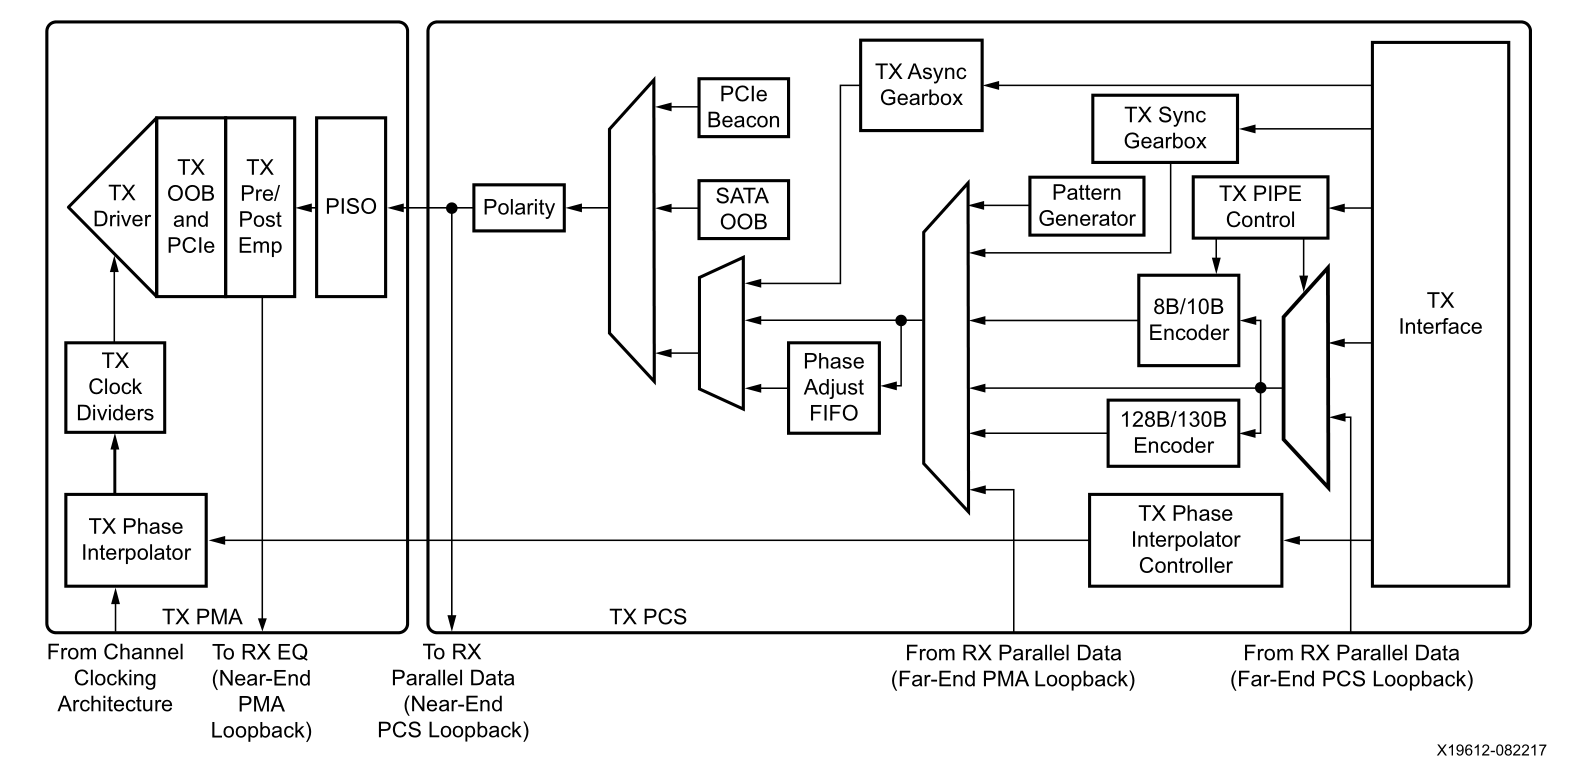
\includegraphics[width=1.2\linewidth]{img/transmitter_block.png}
    \caption{Transmitter Block Diagram~\cite{GTY_guide} }%
    \label{fig:transmitter_block}
\end{figure}

We looked to modify the functionality of a basic implementation of the
transmitter. In the basic implementation a PRBS generator that generates a
sequence through shift registers (as outlined in
Section~\ref{ssub:prbs_generation}) is is fed to the transmitter interface. 

The PRBS module was mainly unchanged from the default with some minor
adjustments.  There were two variations of the PRBS generation module that were
developed.

\subsubsection{Burst Mode over Single Channel}%
\label{ssub:burst_mode_over_single_channel}
Here we modified the PRBS generation module and set it to output zeros if the
enable command was not asserted.  In combination we added a 2 bit register
inside the wrapper, which on overflow toggles the enable flag. This has the
effect of causing the PRBS module to output a sequence interspersed with zeros,
as shown in Figure~\ref{fig:burst_mode_start}. We note also that the full sequence
is transmitted in burst mode (no data is lost).

\begin{figure}[ht]
    \centering
    \hspace*{-3cm}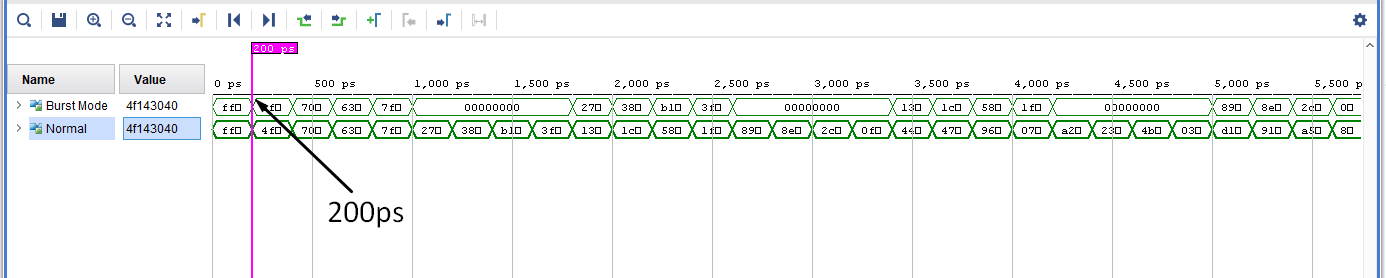
\includegraphics[width=1.5\linewidth]{img/burst_mode_1.png}
    \caption{Single Burst Mode Behaviour}%
    \label{fig:burst_mode_start}
\end{figure}

Comparing Figure~\ref{fig:normal_mode_recur} and
Figure~\ref{fig:burst_mode_recur} we see that the recurrence time (in this simulation we use PRBS7, as
it is a short sequence) for the normal sequence as compared with the burst mode
sequence is about half. This makes sense as the burst mode sequence is
operating on a duty cycle of 50\% and hence should take roughly double the time
to recur.

\begin{figure}[ht]
    \centering
    \hspace*{-3cm}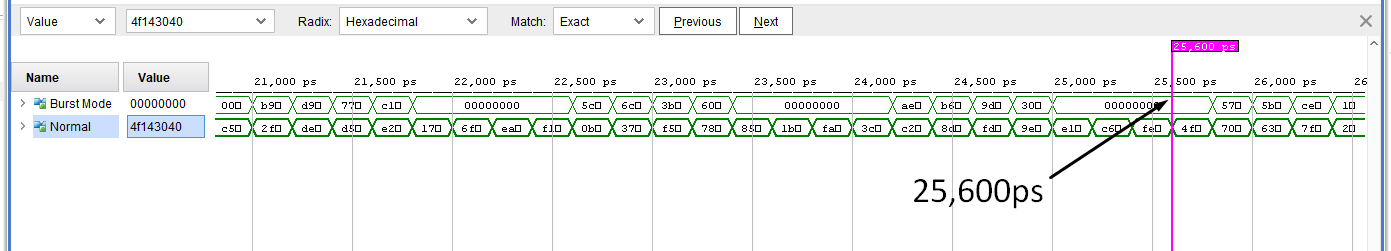
\includegraphics[width=1.5\linewidth]{img/burst_mode_2.png}
    \caption{Normal Mode Recur Time}%
    \label{fig:normal_mode_recur}
\end{figure}

\begin{figure}[ht]
    \centering
    \hspace*{-3cm}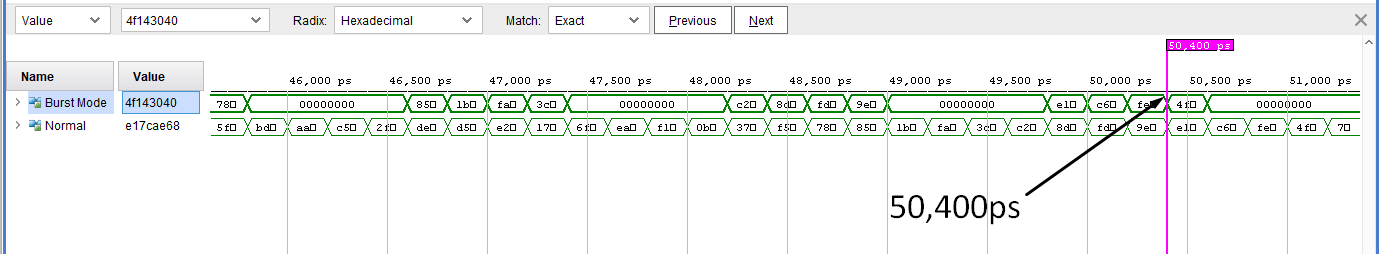
\includegraphics[width=1.5\linewidth]{img/burst_mode_3.png}
    \caption{Burst Mode Recur Time}%
    \label{fig:burst_mode_recur}
\end{figure}

\subsubsection{Switching Between Two Channels}%
\label{ssub:switching_between_two_channels}
Here the PRBS wrapper was changed to feed the two different outputs. The PRBS
generator module was unchanged. Using a 2 bit register which on oveflow
alternated between which of the outputs the PRBS data was sent to, with the
other output being sent zeros. This had the overall effect of having the whole
sequence be sent over two different channels.

\TODO{two channel switch (showing module with two outputs)}


\subsection{Reception}%
\label{sub:prbs_checking}
In normal operation the transceiver would parallise the serial data, and then
pass the data to the PRBS checking module.  
\TODO{image of transceiver -> prbs module}

\subsubsection{Burst Mode Checking}%
\label{ssub:burst_mode_checking}
For burst mode checking there are some issues as there are periods when the
incoming bitstream is all zeros. The PRBS checker module takes the incoming
data as a seed to calculate the next expected sequence. If zeros are provided
then this interferes with the module (as the next expected word will be calculated
based on zeros). To compensate for this we added a register to the wrapper that
would not pass zeros to the checker module. 
In simulation when the PRBS generation module was connected directly to the
PRBS checker this worked correctly, but when passed to through the transceiver,
the checker module would throw errors.  We were not able to determine why.

\subsubsection{Two Channel Checking}%
\label{ssub:two_channel_checking}
In the case where two transmitters were muxed together and were sent to a
single receiver, it should not have been necessary to change the behaviour of
the PRBS checking module.
However we were unable to check this as the lab was closed.

\subsubsection{Disabling The CDR}%
\label{ssub:disabling_the_cdr}
The final step would have been to run the reciever source synchronously. The
transceiver did not allow much flexibilty here. We attemped to do this was by
disabling the CDR and using the same clock to drive the reciever and
transmitter. However the link here was not stable, and we were unable to get
phase readouts that may have allowed us to modify the phase of the incoming
clock. Overall this was unsuccessful.


\section{Optical Transmission}%
\label{optical_transmission}
This part of the project was not completed as the labs were closed before we
were able to test it. However some hardware was prepared, and is described in
the following sections.

\subsection{SOA Board}%
\label{sub:soa_board}
4 PCBs were prepared. The design consisted of an Inphenix SOA mounted in the
center. The electrical component was provided a matched RF line, and the laser
was coupled into the sides. A d-type connecter was also provided so that the
SOA could be temperature controlled.


\subsection{Heatsink and Mount}%
\label{sub:heatsink_and_mount}
It was also necessary to attach a aluminium substrate underneath the PCB board
for heat dissipation. 




